%  This is a Latex template file for articles submitted to 
% SMAI-Journal of Computational Mathematics  
%  It uses the cedram-smai-jcm.cls class file, which is available at 
%          https://ojs.math.cnrs.fr/index.php/SMAI-JCM
%
%  The following template indicates the main features of the class file.
%  In order to avoid mistakes in the handling of meta-data (name, title, etc.),
%  please use all the commands (AND ONLY THOSE) indicated in the preamble for
%  the title and authors.
%

% How to compile:
% pdflatex sample.tex
% bibtex sample
% pdflatex sample.tex
% pdflatex sample.tex

\documentclass[a4paper]
{cedram-smai-jcm}

% Authors may use other style files (e.g., to create figures), as long as
% they do not alter the layout of the article.
\usepackage{tikz}
\usepackage{subcaption}

% Insert here your own definitions, as the following ones:
\newcommand{\bbR}{\mathbb{R}}
\newcommand{\bbC}{\mathbb{C}}
\newcommand{\bbZ}{\mathbb{Z}}

%% Title of the article. 
% The optional argument [] is the short version of the title,
% and the mandatory argument {} the title itself
\title[\LaTeX\ sample SMAI-JCM]{How to use the \emph{SMAI-JCM} class file}

%% Authors, addresses and supports.
% The optional argument is for shortened version appearing in the headings. Please
% distinguish between first, middle and last names with the appropriate commands.
\author[C. Untel]{\firstname{Thierry} \lastname{Untel}}
\address{Inria Sophia Antipolis M\'editerran\'ee, France}
\email{thierry.untel@inria.fr}
\thanks{The first author was supported by the Inria project TEA}

% Repeat the preceding commands for additional authors, commenting out lines
% which should not appear
%Fill in the file as indicated; specific situations (several authors with ) will be handled case by case by the editorial staff.

\author[J. Doe]{\firstname{Jane} \middlename{Q.} \lastname{Doe}}
\address{Department of Mathematics, University of Minnesota, Minneapolis, MN, USA}
\email{doe082@math.umn.edu}

%% Keywords
\keywords{hypersingular integral, multigrid}
  
%% Mathematical classification (2010)
\subjclass{65N35; 15A15}

\begin{document}

% Abstract.
\begin{abstract}
This document is a short user's guide to the \LaTeX\ 
class for articles submitted to \emph{SMAI-JCM}.
The abstract should generally be kept short.
Important: Do not use ``personal'' \LaTeX\ macros in the abstract,
since the text will be extracted for further processing.
\end{abstract}

% Use the \maketitle command after the abstract
\maketitle


%% Beginning of text

% Example of section
\section{Introduction}

Articles may be divided into sections and subsections, like this one.
Shorter articles may not need subsections, while longer articles
can also use subsubsections, and even paragraphs and subparagraphs
(which are unnumbered).

\subsection{Preamble}
Avoid overuse of macros, e.g., mere abbreviations, such as \verb#\bt# to replace
\verb#\begin{theorem}#. The facilities of your editor can be used instead
to minimize keystrokes. Intelligible comments explaining complex
macros may be useful and are appreciated.  Deviations from these
guidelines may cause inaccuracies and delays in the publication.

Avoid overuse of macros.  It is unnecessary to introduce abbreviations,
such as \verb#\bt# to replace \verb#\begin{theorem}#. Instead, the 
facilities of your editor can be used instead
to minimize keystrokes. Intelligible comments explaining complex
macros may be useful and are appreciated.  Deviations from these
guidelines may cause inaccuracies and delays in the publication.

% Example of subsection
\subsection{Header information}

At the start of the paper, after invoking \verb#\title#,  \verb#\author#, \verb#\address#, etc., and
entering the abstract between tags \verb#\begin{abstract}# and \verb#\end{abstract}#,
invoke the \verb#\maketitle# command to typeset this header information.

\subsection{References}

The bibliography must be built using bibtex. A sample of a bibtex file,
\texttt{biblio.bib},
is included as part of this sample manuscript and is available on the journal website
%% see the \url command
\url{https://ojs.math.cnrs.fr/index.php/SMAI-JCM}.

References are entered into the bibtex file as in the sample
and then citations are made in the article text by using the \verb#\cite# command.
Here are examples of an article \cite{LL}, a book \cite{ARN}, a PhD thesis 
\cite{VAJ}, an unpublished paper \cite{MSIADOC}, and a book section \cite{KT}.


\section{Figures}

Figures must be provided in PDF.  The following commands
illustrate how to include a figure in the text.

\begin{verbatim}
\begin{figure}[tbp]
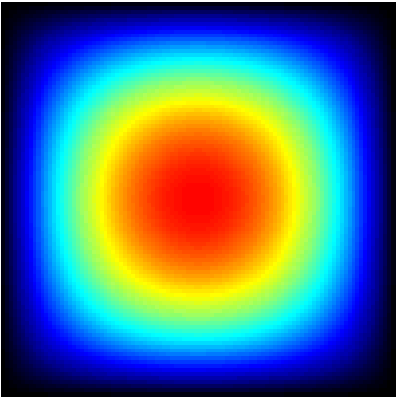
\includegraphics[width=0.3\linewidth]{figure-msia.pdf}
\caption{Example of figure.}
\label{exfig}
\end{figure}
\end{verbatim}
The width parameter, which is \verb#0.3\linewidth# here, can be adjusted
as needed, but should not exceed \verb#1.0\linewidth#.
See Figure~\ref{F1} for an example.
Subfigures can be used as well, as shown in Figure~\ref{F2}.

\begin{figure}[!htbp]
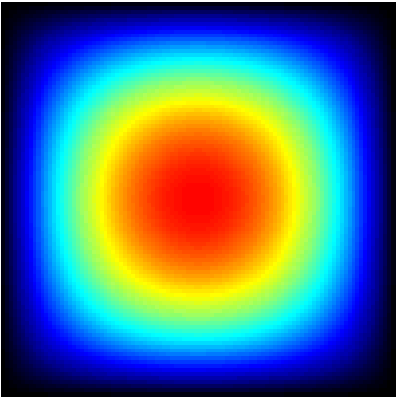
\includegraphics[width=0.3\linewidth]{figure-msia.pdf}
\caption{Example of figure.}
\label{F1}
\end{figure}


\begin{figure}[!htbp]
  \centering
  \begin{subfigure}[b]{0.45\textwidth}
    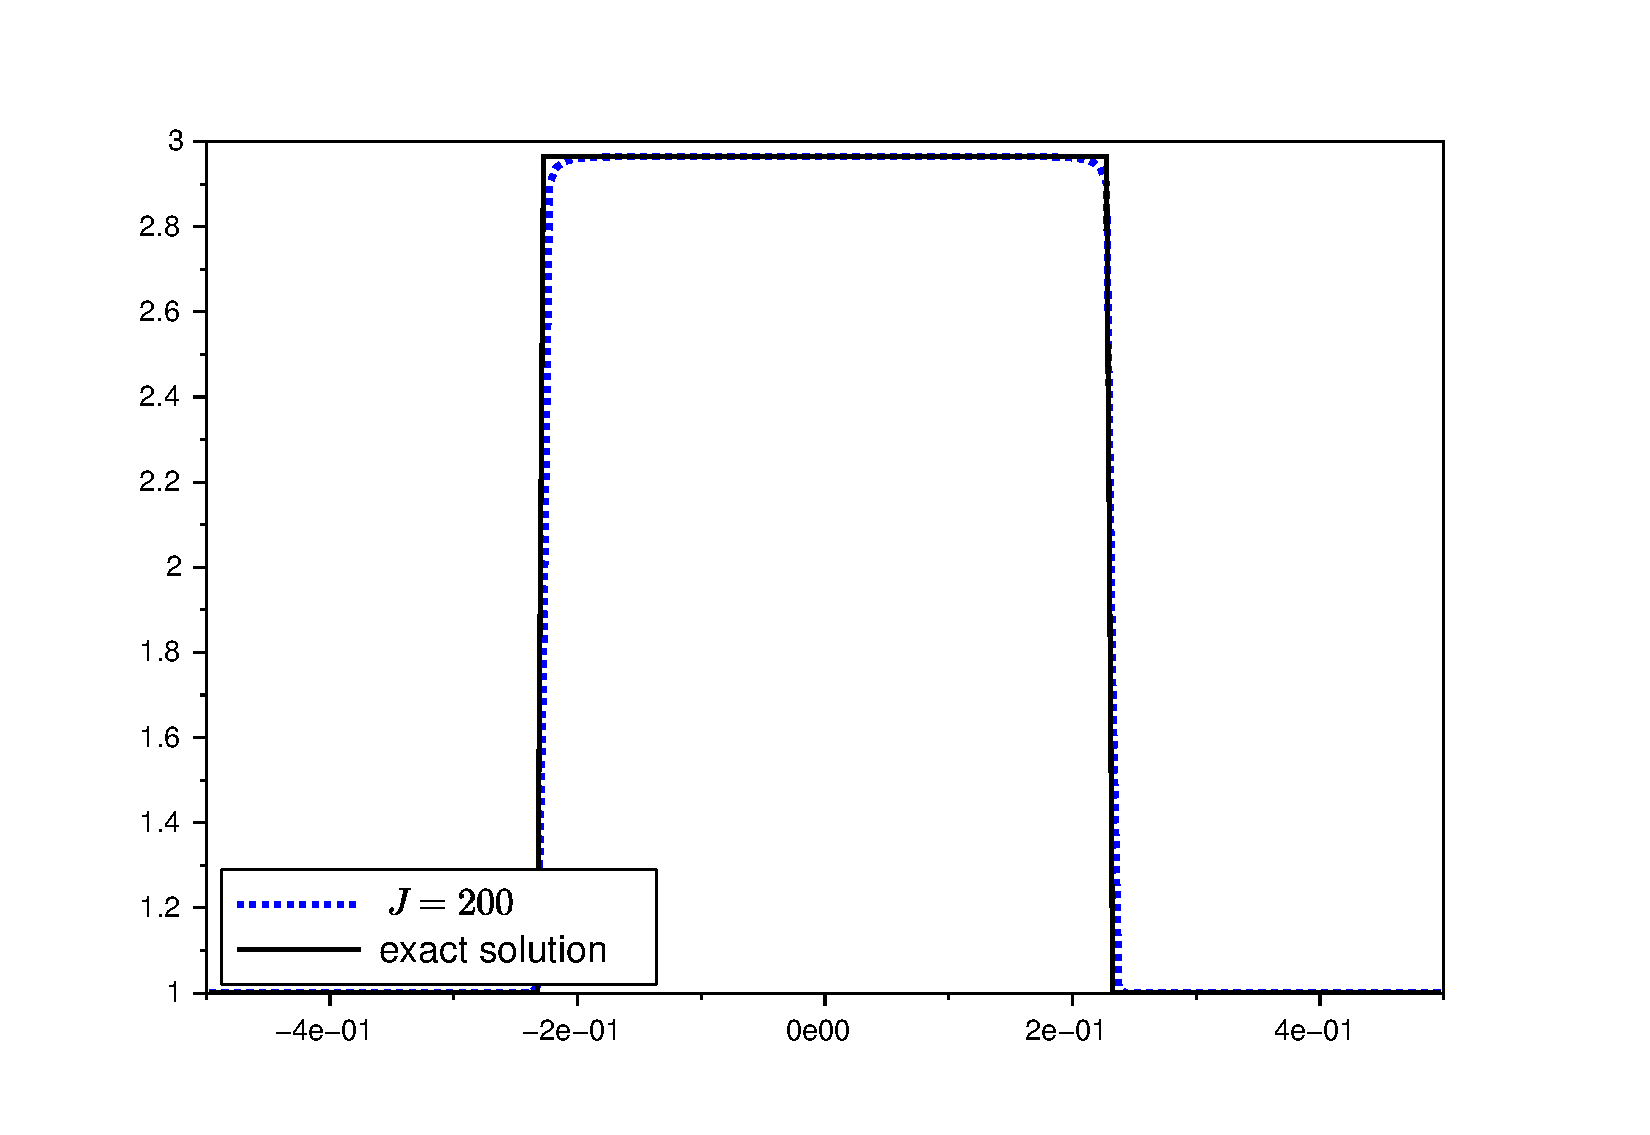
\includegraphics[clip,trim=64 40 90 60,scale=0.34]{./Density_Rhos3J200Dt4044e-9}
    \subcaption{Volume fraction}
  \end{subfigure}
  \quad
  \begin{subfigure}[b]{0.45\textwidth}
    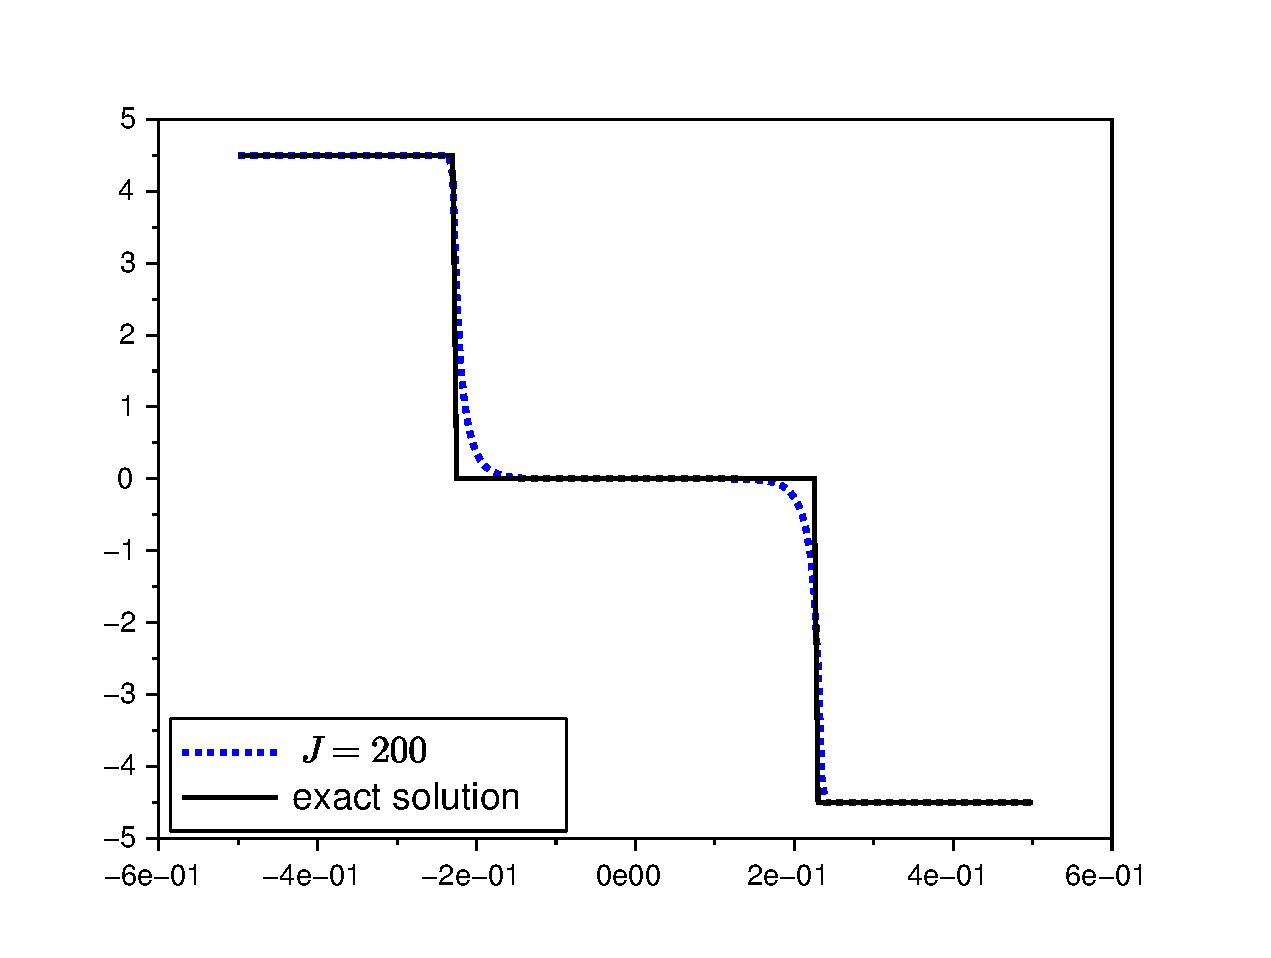
\includegraphics[clip,trim=45 30 60 50,scale=0.4]{./Velocity_Rhos3J200Dt4044e-9}
    \subcaption{Velocity}
  \end{subfigure}
  \caption{Exact and numerical ($J=200,\ \Delta t=4.044\ 10^{-6}$) solution
  at $t=1$ with $U = 4.5$}
\label{F2}
\end{figure}

Besides figures in the text, SMAI-JCM allows for the possibility of publishing
additional supplementary materials in various format, for example, animations.
Contact the editors-in-chief if you would like to explore this possibility.

%To refer to a specific definition, theorem, etc., put \label{labelname} inside
%the corresponding environment and use \ref{labelname} in text to point to this
%definition, theorem, etc.

\section{Proclamation environments}

Environments are defined for theorems, lemmas, proofs, etc.
These include \verb#theorem#, \verb#lemma#, \verb#corollary#,
\verb#proposition#, \verb#definition#, \verb#remark#, \verb#remarks#,
\verb#notation#, \verb#example#, and \verb#proof#.

Here is an example of a numbered equation, then a theorem, followed by the proof.
We define degrees of freedom 
\begin{equation}\label{dofs}
\xi(u) = \int_e uq, \quad q\in \mathcal P_{r-2}(e),\quad e\in \Delta(T).
\end{equation}
The following theorem establishes their unisolvence.

\begin{theorem}\label{th:true}
  For any integers $r,n\ge 1$ and any $n$-simplex $T$, the degrees of
  freedom \eqref{dofs} are unisolvent on $V(T)=\mathcal P_r(T)$.
\end{theorem}

\begin{proof}
  It suffices to verify, first, that the number of degrees of freedom proposed
  for $T$ does not exceed $\dim V(T)$, and, second, that if all the degrees of
  freedom vanish when applied to some $u\in V(T)$, then $u\equiv 0$. \\
  For the first claim, we have note that
  the total number of degrees of freedom is at most
$$
\sum_{d=0}^n\#\Delta_d(T)\dim\mathcal P_{r-d-1}(\mathbb R^d)=
\sum_{d=0}^n\binom{n+1}{d+1}\binom{r-1}{d}=\binom{n+r}{n}=\dim\mathcal P_r(T).
$$
The second claim can be established by induction on the dimension.
\end{proof}

Illuminating examples and remarks make a paper more appealing.

\begin{example}\label{ex:good}
  This is an example of an example.
\end{example}

\begin{remark}
  The mathematics in this paper is just for illustration purposes.  It is not
  intended to make sense.
\end{remark}

Now consider a result like this one.

\begin{lemma}\label{lemm:call}
  The energy content $E$ of an object of rest mass $m$ satisfies $E\le 2 m c^2$.
\end{lemma}

\noindent
If its proof is separated from the statement of the result
we can use the \verb#ProofOf# environment to tag the
delayed proof.

\medskip

\begin{ProofOf}{Lemma \ref{lemm:call}}
  This follows from Einstein's mass--energy relation and the inequality $1\le 2$,
  whose proof is left to the reader.
\end{ProofOf}


\appendix

\section{An appendex on appendices}

The paper can contain an appendex, for instance to detail a proof, or even multiple appendices.

\section{Further boring but useful stuffs}
Note that appendex sections have labels specific to that section.

\begin{equation}
E\ge 0.5 m c^2.
\end{equation}


\section*{Acknowledgements}
We get by with a little help from  our friends.
(The \verb#\thanks# tag in the header is used for acknowledging the support of institutions,
this section for thanking persons.

% The next command determines the bibliography style. Please do not
% change this.
\bibliographystyle{plain}

%  This includes the bib file
\bibliography{biblio}

\end{document}










